\documentclass[spanish,notitlepage,letterpaper,11pt]{article} % para artÌculo en castellano
\usepackage[utf8]{inputenc} % Acepta caracteres en castellano
\usepackage[T1]{fontenc} % font encoding
\usepackage[spanish]{babel} % silabea palabras castellanas
\usepackage[none]{hyphenat} 
\usepackage{amsmath}
\usepackage{color}
\definecolor{labelcolor}{RGB}{100,0,0}
\usepackage{amsfonts}
\usepackage{amssymb}
\usepackage[colorlinks=true,urlcolor=blue,linkcolor=blue]{hyperref} % navega por el doc
\usepackage{graphicx}
\usepackage{geometry} % See geometry.pdf to learn the layout options.
\geometry{letterpaper}  % ... or a4paper or a5paper or ... 
%\geometry{landscape}  % Activate for for rotated page geometry
%\usepackage[parfill]{parskip} % Activate to begin paragraphs with an empty line rather than an indent
\usepackage{epstopdf}
\usepackage{fancyhdr} % encabezados y pies de pg
\usepackage{lineno}
%\linenumbers

\pagestyle{fancy} 
\chead{\bfseries Caos y péndulo doble} 
\lhead{\it L.A Núñez  } % si se omite coloca el nombre de la seccion
\rhead{Octubre 2020} 
\lfoot{Escuela de Física} 
\cfoot{Universidad Industrial de Santander} 
\rfoot{\thepage} 

\voffset = -0.25in 
\textheight = 8.0in 
\textwidth = 6.5in
\oddsidemargin = 0.in
\headheight = 20pt 
\headwidth = 6.5in
\renewcommand{\headrulewidth}{0.5pt}
\renewcommand{\footrulewidth}{0,5pt}
\DeclareGraphicsRule{.tif}{png}{.png}{`convert #1 `dirname #1`/`basename #1 .tif`.png}



\begin{document}
\title{Caos y el péndulo doble \\ 
Un problema de valores iniciales}
\author{
\textbf{Luis A. Núñez} \\ 
\textit{Escuela de Física} \textit{Universidad Industrial de Santander} \\ 
\textit{Bucaramanga, Colombia}
}
\date{\today}
\maketitle
%\tableofcontents
\begin{abstract}
    Presentamos una propuesta de experimento numérico para explorar el caos determinísta. El sistema mecánico será el péndulo doble  
\end{abstract}

\section{El problema}
\textbf{Explorar la evolución de las variables dinámicas de un péndulo doble}
El péndulo doble es un sistema como se muestra en la figura \label{Pendulo2}: dos masas $m_1$ y $m_2$ atadas a dos varillas sin masas de longitudes $l_1$ y $l_2$, respectivamente. 
\begin{figure}[ht!]
\centering
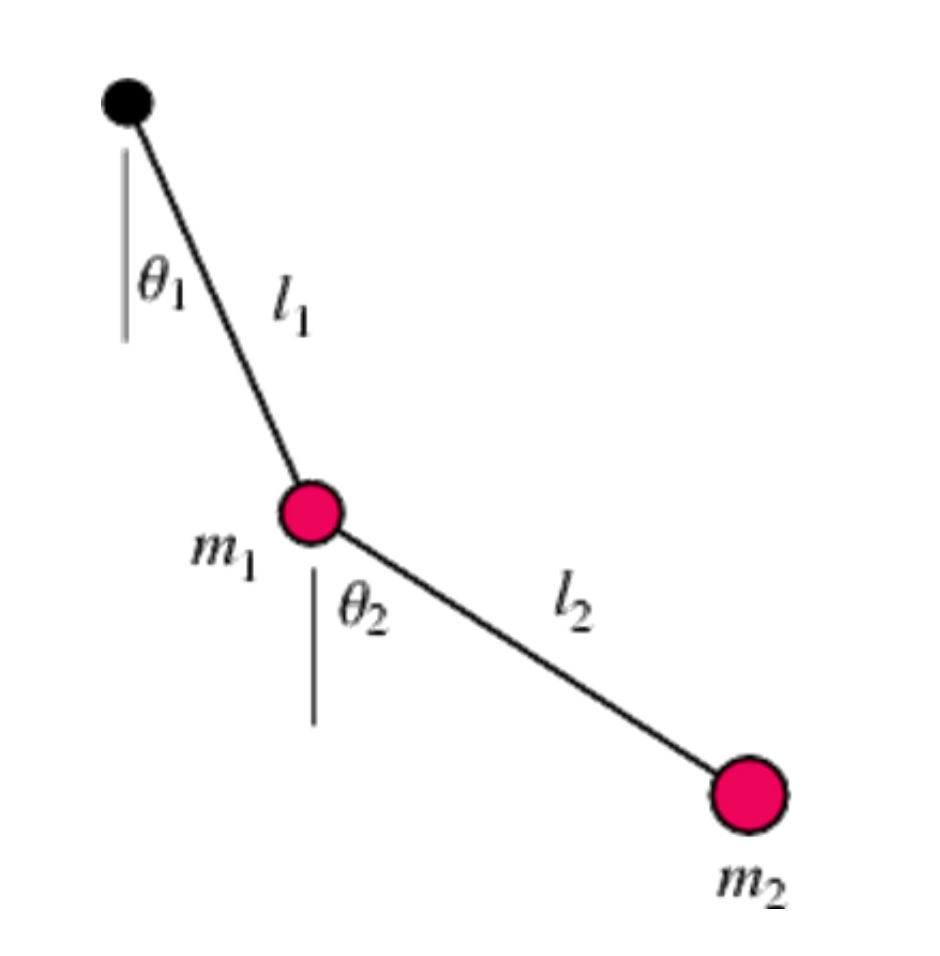
\includegraphics[width=2in]{Figuras/Pendulo2.png}
\label{Pendulo2}
\end{figure}

Consideremos las siguientes ecuaciones diferenciales ordinarias de segundo orden que describen la dinámica del sistema antes mencionado:
\begin{equation}
\ddot{\theta}_1 = \frac{g({\rm sen}~\theta_2\cos \Delta \theta -M{\rm sen}~\theta_1 ) -(l_2 \dot{\theta}_2^2 + l_1 \dot{\theta}_1^2\cos \Delta \theta){\rm sen}\Delta \theta}
{l_1(M -\cos^2 \Delta \theta)}
\label{ddtheta1}
\end{equation}
\begin{equation}
\ddot{\theta}_2 = \frac{gM({\rm sen}~\theta_1\cos \Delta \theta -{\rm sen}~\theta_2 ) -(M l_1 \dot{\theta}_1^2 + l_2 \dot{\theta}_2^2\cos \Delta \theta){\rm sen}\Delta \theta}
{l_2(M -\cos^2 \Delta \theta)} \, .   
\label{ddtheta2}
\end{equation}
Donde $M \equiv 1 + m_1/m_2$ y $\Delta \theta = \theta_1 -\theta_2$. 

\begin{enumerate}
    \item A partir del sistema de ecuaciones diferenciales (\ref{ddtheta1}) y (\ref{ddtheta2}), construya un sistema de cuatro ecuaciones diferenciales de primer orden 
    \item Intégrelo numéricamente, tanto para pequeñas como para grandes amplitudes. 
    \item Valide el comportamiento de su integración con los simuladores disponibles en línea, i.e. \\ \url{https://www.myphysicslab.com/pendulum/double-pendulum-en.html}
    \item ¿Cuándo y por qué el sistema muestra el comportamiento caótico? Discuta el espacio de condiciones iniciales para el cual el sistema presenta ese comportamiento caótico
    \item Analice el comportamiento de su señal en términos del un espectro de potencias de Fourier y de la huella en un espectrograma, para grandes y pequeñas amplitudes. ¿qué puede concluir de ambos comportamientos?
    \item Linealice el sistema. Esto es: considere $\theta_1 << 1$,  $\theta_1 << 1$ y $\theta_1^2 \sim \theta_1^2 \sim 0$, ${\rm sen}~\theta_1 \sim \theta_1$, ${\rm sen}~\theta_2 \sim \theta_2$, $\cos\theta_1 \sim 1 $ y $\cos\theta_2 \sim 1 $. Muestre que las ecuaciones (\ref{ddtheta1}) y (\ref{ddtheta2}) se reducen al siguiente sistema de ecuaciones
    \begin{equation}
\ddot{\theta}_1 \approx \frac{g(\theta_2 -M\theta_1)}{l_1(M -1)} \quad {\rm y} \quad \ddot{\theta}_2 \approx \frac{gM\Delta \theta}{l_2(M -1)}
\label{aproxddottheta}
    \end{equation}
    \item Estime la transición entre pequeñas oscilaciones y grandes amplitudes. Esto es, para cuales amplitudes la integración del sistema (\ref{ddtheta1}) y (\ref{ddtheta2}) reobtiene el sistema (\ref{aproxddottheta}).
    \item Compare el comportamiento del espectro de potencias y el espectrograma para ambos sistemas de ecuaciones diferenciales.
\end{enumerate}

Mayores detalles de los conceptos y las ecuaciones que describen este sistema se encuentran en: 
\begin{itemize}
    \item \url{https://en.wikipedia.org/wiki/Double_pendulum}
    \item \url{http://scienceworld.wolfram.com/physics/DoublePendulum.html}
\end{itemize}

Descripciones de la evolución de este sistema están en muchos videos y simuladores. Son particularmente buenos y recomendables los siguientes videos
\begin{itemize}
    \item \url{https://www.youtube.com/watch?v=fDek6cYijxI}
    \item \url{https://www.youtube.com/watch?v=pEjZd-AvPco}
\end{itemize}

%\bibliographystyle{unsrt}
%\bibliography{EstimaRoce}
\end{document}
